\documentclass[11pt]{article}
\usepackage{geometry}
\geometry{letterpaper}
\usepackage[parfill]{parskip} 
\usepackage{graphicx}
\usepackage{amssymb}
\usepackage{float}

\title{CSCI503: Parallel Programming / Homework 1}
\author{Zhitao Zhou Student}

\begin{document}

\maketitle

\section{Discussion Question}
\begin{enumerate}
\item[Q1]Write a paragraph on your background, your interests in parallel programming, and what you hope to get out of taking this course

I am pursuing master degree of Computer Science with specialization in high-performance and simulation. I have done some research project in GPU programming with OpenCL and CUDA. I am very interested in parallel programming for an increasing number of companies are building their application on multi-core computers and clusters to improve processing speed of request from user and software performance with workstation. So parallel programming is a must-have skill for software engineer in the future. I hope to get more hand-on experience with parallel programming and get familiar with the cutting-edge parallel programming model and algorithm design technique out of taking this course.     
 
\item[Q2]
According to the November 2014 Top 500 Ranking,
\begin{enumerate}
\item The machine with maximal number of processors ranked number 1 which has 3,120,000 processors, and the machine with minimal number of processors has 2,992 processors.
\item The best computing performance is 33,862,700 GFlop/s, and the worst computing performance is 153,381 GFlop/s.
\item 
The following table on page ~\pageref{table:table1} are system from different vendors.

\begin{table}[ht]
\label{table:table1}
\caption{The number of systems from different vendors}
\begin{tabular}{ll}
Vendors                         & Count \\
AMD, ASUS, FIAS, GSI            & 1     \\
Acer Group                      & 1     \\
Adtech                          & 1     \\
Clustervision/Supermicro        & 1     \\
HP/WIPRO                        & 1     \\
Hitachi/Fujitsu                 & 1     \\
IPE, Nvidia, Tyan               & 1     \\
Inspur                          & 1     \\
Intel                           & 1     \\
NEC/HP                          & 1     \\
NRCPCET                         & 1     \\
Netweb Technologies             & 1     \\
Niagara Computers, Supermicro   & 1     \\
PEZY Computing / Exascaler Inc. & 1     \\
Supermicro                      & 1     \\
Xenon Systems                   & 1     \\
ClusterVision                   & 2     \\
Dawning                         & 2     \\
Hitachi                         & 2     \\
Itautec                         & 2     \\
Oracle                          & 2     \\
Self-made                       & 2     \\
T-Platforms                     & 2     \\
Atipa                           & 3     \\
MEGWARE                         & 3     \\
NEC                             & 3     \\
RSC Group                       & 4     \\
NUDT                            & 5     \\
Fujitsu                         & 8     \\
Dell                            & 9     \\
Bull                            & 18    \\
SGI                             & 23    \\
Cray Inc.                       & 62    \\
IBM                             & 153   \\
HP                              & 179  
\end{tabular}
\end{table}

\item 51\% of the systems are for industry,   17.6\% of the systems are for academic purpose, 4.6\% of the systems are for government, 3\% of the systems are for vendors, 23.6\% of the systems are for research and 0.2\% of the systems are for others.
\item USC HPCC system ranked 94 in the list.
\end{enumerate}

\item[Q3]
\begin{enumerate}
\item when $i=1$,$N=2$ and sequential cost is $0.15$,the bound of speedup is [1,1.7392]
\item when $i=2$,$N=4$ and sequential cost is $0.3$, the bound of speedup is [1,2.1053]
\item when $i=3$,$N=8$ and sequential cost is $0.45$, the bound of speedup is [1,1.9277]
\item when $i=4$,$N=16$ and sequential cost is $0.15$, the bound of speedup is [1,4.9231]
\end{enumerate}

\item[Q4]
\begin{enumerate}
\item There are 5760 processors on the device.
\item The memory units are organized as Shared Memory, Register, Local Memory, Global Memory, Constant Memory, Texture Memory.
\item The base clock is 705MHz, and the boost clock is 876 MHz.
\item The memory speed is 7.0 Gbps
\end{enumerate}

\item[Q5]
If job(i) is executed in sequential order, we need to launch one process whose overhead is 1 microsecond and we need to run 500 loops and each cost 20 microseconds, so the total time cost is $1+20*500=10001$ microseconds.

If job(i) is executed in parallel, we need to sequentially launch 500 processes , whose overhead is 500 microseconds, and all processes ends when the last initiated processes finishing executing, so the total time cost is $500+20=520$ microseconds.

The speedup of parallel with sequential executing is $10001/520 = 19$. 

\item[Q6]
The reason will the result is not reproducible is that in threadFunction, it adds a local variable to a global variable, which entails data dependency problem. One thread may be writing this global variable while other thread is writing this variable, causing some local result is lost. There are two ways to remedy this problem. One is using atomic operation. Let anything instruction involving this global variable to be atomic, then no thread can writing this variable until other variable finish writing this variable. The other approach is use reduction. We can store the result from each thread in an array, and use one iteration to sum all the local result.

\end{enumerate}
\section{Programming Question}
\begin{figure}[H]
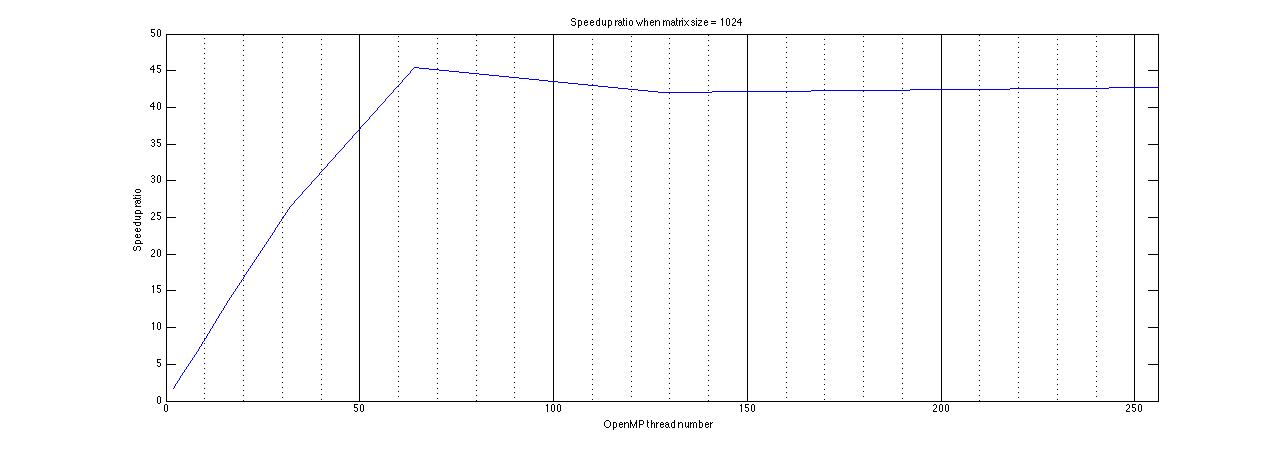
\includegraphics[scale=0.4]{speedup}
\centering
\end{figure}
\begin{figure}[H]
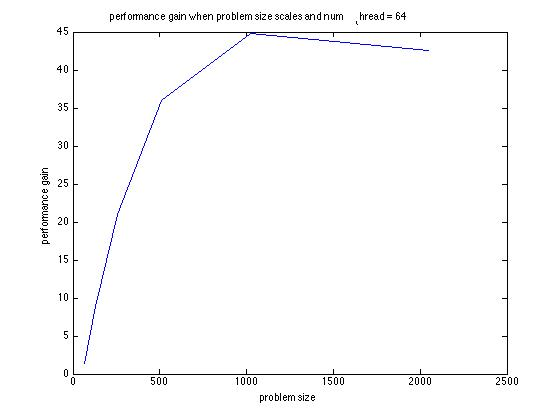
\includegraphics[scale=0.8]{perf}
\centering
\end{figure}
I do time experiment on aludra.usc.edu. 
\begin{enumerate}
\item The computer has 16 cores.
\item After using 64 threads,from the first image, I stop seeing performance improving.
\item From second figure, when we scale the problem size, we have performance gain. The reason is the performance gain is decided by the equation $perf=1/((1-p)+(p/N))$. Because I implemented the matrix multiplication as one process will process one row of elements in the final result, which is 1D blocked data layout. Assume the problem size is $n$. The percentage of arithmetic operation which is not parallel executed is $2n^2/(2n^3)=1/n$. So the speedup is given by $1/((1-1/n)+1/(nN))$. With N is fixed to 64 and n is increasing, this value is ascending, so the speedup is ascending. But this estimate is very rough. We can see from both image that when we use 64 threads, the performance stop improving, then this bound is decided by other factors. The reading latency of matrix B may be the bounding factor. And the overhead of OpenMP thread forking and implicitly synchronizing may also be the bounding factor. And this is the result i expected. Since we cannot get unlimited performance with certain machine.  
\end{enumerate}
\end{document}
